% CREATED BY DAVID FRISK, 2016
\chapter{Theory}
This chapter will present the theory that is relevant to construct a client and server verifiable VAHSS construction.  First the \textit{preliminaries} needed is described, this includes notation that is used, theorems/definitions, assumptions and several cryptographic preliminaries and  concepts. Then the VAHSS construction, which this reports aims to extend to include verification of clients honesty, originally described in \cite{SumItUp,VAHSS} is presented.  Finally two different range proof constructions is described in detail. These two constructions will be refereed to as \textit{signature-based range proof} and \textit{bulletproof}. 


\section{Cryptographic preliminaries}
This sections aim to present all relevant background to the cryptographic constructions presented in section \ref{sec:VAHSS} and \ref{sec:RF_theory}. 
\subsection*{Notation and setup}
First lets define some notation that will be used trough out the paper.
Consider $n$ clients and $m$ servers, to simplify notation define the two sets $\mathcal{N}=\{1,...,n\}$ and $\mathcal{M} = \{1,...,m\}$. Let $c_i$ and $x_i$ for $i\in\mathcal{N}$ denote the clients (data providers) and their respective data. Denote the servers by $s_j$, where $\:j\in\mathcal{M}$.


Let $\mathds{F}=\mathds{Z}_N$ denote a finite field, where $N$ is a large prime and let $\mathds{G}$ denote he unique subgroup of order $q$.  Define $g\in\mathds{G}$ to be a group generator and $h\in\mathds{G}$ a group element such that no one knows $log_g\:h$. The two group elements $g,h$ can either be chosen by a trusted party or by one of the participates using a \textit{coin-flipping} protocol \cite{pedersen}.

The notation $x\in_R\mathds{Y}$, means that an element $x$ in chosen at random from the set $\mathds{Y}$.

\subsection*{Definitions and theorems}

\begin{Mydef}[\textbf{Euler's totient function}]
The function $\Phi(n)$ is defined as the counter of the number of integers that are relative primes to $n$ in the set $\{1,...,n\}$ . Note if $n$ is a prime number $\phi(n) = n-1$.
\end{Mydef}
\vspace{10pt}
\begin{thm}[Euler's Theorem]
\label{thm:euler}
For all integers $x$ and $n$ that are co-prime it holds that:
$x^{\Phi(n)} = 1\:( \text{mod n})$, where $\Phi(n)$ is Euler's totient function.
\end{thm}
\vspace{10pt}
From Theorem \ref{thm:euler} it follows that for arbitrary $y$ it holds that $x^{y\Phi(n)} = 1 \:( \text{mod n})$.
\vspace{10pt}
\begin{Mydef}[Pseudorandom Function (PRF)]
ehjs
\end{Mydef}

\subsection*{Assumptions}
In this section cryptographic assumptions that is used in the constructions presented later rely on will be presented. A remark is that this assumptions will not hold in the presence of quantum computers which means that the constructions presented here is not secure post quantum.
\\
\begin{Ass}[\textbf{Discrete logarithmic assumption}]
Let $\mathds{G}$ be a group of prime order $q$, a generator $g\in \mathds{G}$ and an arbitrary element $y \in\mathds{G}$, it is  infeasible to find $x \in \mathds{Z}_q$, such that $y=g^x$
\end{Ass}
\vspace{10pt}
\begin{Ass}[\textbf{q-strong Diffie Hellman Assumption}]
 Given a group $\mathds{G}$, a random generator $g\in \mathds{G}$ and powers $g^x,...,g^{x_q}$, for $x \in_R \mathds{Z}_p$ and  $q= |\mathds{G}|$. It is then  infeasible for an adversary to find $(c, g^{\frac{1}{x+c}})$, where $c \in \mathds{Z}_p$.
\end{Ass}

%\begin{Ass}[RSA Assumption]
%Given modolus $n$, exponent $e$ and cipher text $c$ it is believed to be intractable to find $m$ such that $c= m^e \:(\text{mod n})$.
%\end{Ass}


\subsection*{Homomorphic Secret Sharing}
Secret sharing \cite{How_share_A_secret} is a method where a secret is to split  into shares to hide its value. A secret $x$ is split into $m$ shares $x_i \text{ s.t } i\in\{1,...,m\}$, where any the shares reviles no information about the original secret $x$. To reconstruct the value $x$ one have to combine at least $\tau$ shares and any subset of shares smaller than $\tau$ reviles no information about the original secret $x$, this is called a $(\tau,m)$-threshold scheme. In this paper $\tau = \textit{number of shares}=m$. Further this paper will consider additive secret sharing scheme, thus the shares will have the property; $x = \sum_{i=1}^\tau x_i$. 

\subsection*{Homomorphic hash functions}
Let $\mathcal{H}$ be a cryptographic hash function, $\mathcal{H}:\mathds{F}\to \mathds{G}$. Any such function should satisfy the following two properties:
\begin{itemize}
    \item \textbf{Collision-resistant} It should be hard to find $x,x'\in\mathds{F}$ such that $x\neq x'$ and $\mathcal{H}(x)=\mathcal{H}(x')$.
    \item \textbf{One-Way} It should be computationally hard to find $\mathcal{H}^{-1}(x)$.
\end{itemize}

A homomorphic hash function should also satisfy the following property:
\begin{itemize}
    \item \textbf{Homomorphism} For any $x,x'\in\mathds{F}$ it should hold that $\mathcal{H}(x\circ x') = \mathcal{H}(x)\circ\mathcal{H}(x')$. Where $\circ$ is either $"+"$ or $"*"$.
\end{itemize}

A such function satisfying the thee properties is $\mathcal{H}_1(x):\mathds{F}\to\mathds{G}$ and $\mathcal{H}_1(x)= g^{x}$ \cite{HHF}. 
\subsection*{Pedersen Commitment scheme}
Define a commitment to an $x\in\mathds{F}$ as $\mathds{E}(x,R)=g^xh^R$, where $R\in_R\mathds{F}$, this commitment is known as \textit{Pedersen commitment} and originally presented in \cite{pedersen}. This commitment satisfies the following theorem;
\\
\begin{thm}
\label{thm:C=g^xh^R}
For any $x\in\mathds{F}$ and for $R\in_R\mathds{F}$, it follows that   $\mathds{E}(x,R)$ is uniformly distributed in $\mathds{G}$. If we have two commits satisfying $\mathds{E}(x,R)=\mathds{E}(x',R')$  $x\neq x'$ and  $x\neq x'$ then it must hold that $R\neq R' \:\text{mod}\:q$ and 
\begin{equation*}
    log_g(h) = \frac{x-x'}{R'-R} \text{ mod }N.
\end{equation*}
\end{thm}
\begin{proof}
The statements of the theorem follows from solving for $log_g(h)$ in $\mathds{E}(x,R)=\mathds{E}(x',R')$ 
\end{proof}

Theorem \ref{thm:C=g^xh^R} implies that if someone knows the discrete logarithm of $h$ with respect to $g$, i.e $log_g(h)$, he is able to provide two equal commits, $\mathds{E}(x,R)=\mathds{E}(x',R')$ such that $x\neq x'$. Note that in he set up of the protocol it was required that this logarithm should be unknown to any party and generated by a trusted third party or by one of the participants using a coin-flipping protocol.

Further note that Pedersen commitment is homomorphic. Hence for arbitrary messages $x_1,x_2\in\mathds{F}$, random values $R_1,R_2\in_R\mathds{F}$ and the commits $C_i=\mathds{E}(x_i,R_i),\:i\in\{1,2\}$, it holds that $C_1\cdot C_2 = \mathds{E}(x_1+x_2,R_1+R_2)$.

A final remark is the similarity between the hash function $\mathcal{H}_1$ and the Pedersen commitment $\mathds{E}$, the hash function can be seen as a generalisation of the Pedersen commitment. 

\subsubsection*{Vector Pedersen Commitment scheme}
\subsection*{Bilinear mapping}
\label{sec:bilinear}

\subsection*{Zero knowledge proof}
Zero-knowledge proofs  (ZKP) was first presented in \cite{OG_ZKP}. A ZKP consist of two parties: \textit{Prover} \& \textit{Verifier} and satisfies the properties  in Definition \ref{def:ZKP}. After successfully performing a ZKP the prover has convinced the verifier that a certain statement of a secret $x$ is true without having relieved any other information about $x$. This is done by providing a witness $w$ of the statement. In this paper ZKP that ensures proof of knowledge (PoK) is of interest,  this means that the verifier is now only convinced that the statement is true but also that the prover knows the value of secret $x$.  Further this paper will study zero knowledge range proof (ZKRP) where the statement that the prover convinces the verifier of is that the value of secret belongs to a predetermined interval.

\begin{Mydef}
\label{def:ZKP}
A ZKP should fulfill the three properties: 
\begin{itemize}
\item \textbf{Completeness} 
\item \textbf{Soundness} 
\item  \textbf{Zero-knowledge}
\end{itemize}
\end{Mydef}

\subsection*{Fiat-Shamir heuristic}
 Fiat-Shamir heuristic \cite{Fiat-Shamir} can be used to convert an interactive protocol  non interactive, here it will be used to construct non-interactive ZKP. A non interactive constructions for a zZKP requires no communication between the prover and verifier during the construction of the proof. In interactive constructions the verifier sends a challenge $c\in_R\mathds{F}$ to the prover which is included in the proof to convince the verifier of its correctness. The Fiat-Shamir heuristic uses a challenge that instead of being randomly chosen by the verifier is the a hash of the transcripts up to this point. This heuristic convert an interactive protocol to a non-interactive while preserving its secure and full zero-knowledge in the random oracle model (ROM). 

\section{Verifiable additive homomorphic secret sharing}
\label{sec:VAHSS}
This section will describe the verifiable additive homomorphic secret sharing (VAHSS) constructions presented in \cite{VAHSS,SumItUp}. Lets assume  $n$ clients/data providers and $m$ servers. Each client split their secret $x_i$ into $m$ shares, $x_{ij}$ and sends one share to each server. The servers receives shares from all $n$ clients and computes the partial function $y_j = \sum_{i=1}^n x_{ij} $ and publishes the result. The final result $y = \sum_{j=1}^m y_j$ can then be computed by any party. In verifiable additive homomorphic secret sharing a proof $\sigma$ that verifies that $y= \sum_{j=1}^n y_j= \sum_{j=1}^m \big( \sum_{i=1}^n  x_{ij} \big) =  \sum_{i=1}^n \big( \sum_{j=1}^m  x_{ij} \big)  = \sum_{i=1}^n x_i$ is generated and published. This allows any party to verify the correctness of the severs computations. Remark that the individual secrets $x_i$ is never revealed in the protocol.


\subsection*{Construction}
In this section a VAHSS construction  is presented. The construction consists of the six PPT algorithms: \textbf{ShareSecret}, \textbf{PartialEval}, \textbf{PartialProof}, \textbf{FinalEval}, \textbf{FinalProof} and \textbf{Verify}. The clients/data providers executed the step \textbf{ShareSecret}, the servers \textbf{PartialEval} and \textbf{PartialProof} and the last three steps can run by anyone. The complete construction looks like:

\begin{algorithm}[H]
\caption{\textbf{: Verifiable additive homomorphic secret sharing}}
\begin{itemize}
  \item\textbf{ShareSecret $(1^\lambda,i,x_i)\xrightarrow[]{}(\pi_i,\{x_{ij}\}_{j\in\mathcal{M}})$}\\
Pick uniformly at random $\{a_i\}_{i\in\{1,..,t\}}\in\mathds{F}$ and a $t$-degree polynomial $p_i$ on the form $p_i(X) = x_i + a_1X+...+a_tX^t$. Let $H:x\to g^x$, (g generator the multiplicative group of $\mathds{F}$), be a collision-resistant homomorphic hash function. Let $R_i\in\mathds{F}$ be the output of a PRF. We require $R_n\in \mathds{F}$ to satisfy
$R_n = \phi(N)\lceil \frac{\sum_{i=1}^{n-1}R_i}{\phi(N)}\rceil- \sum_{i=1}^{n-1}R_i $. Compute $\tau_i = H(x_i+R_i)$, and put $x_{ij}=\lambda_{i,j}p_i(sigma_{ij})$. \\
The algorithm published $\pi_i$ and sends $x_{i,j}$ to server $j$ for $j\in\mathcal{M}$. 

\item\textbf{PartialEval $(j,\{x_{ij}\}_{i\in\mathcal{N}})\xrightarrow[]{}y_j$}\\
Compute and publish $y_j = \sum_{i=1}^n x_{ij}$.

\item\textbf{PartialProof $(j,\{x_{ij}\}_{i\in\mathcal{N}})\xrightarrow[]{}\sigma_j$}\\
Compute and publish $\sigma_j = \prod_{i=1}^n g^{x_{ij}} =  g^{\sum_{i=1}^n x_{ij}}= g^{y_j}=H(y_j)$.

\item\textbf{FinalEval $(\{y_j\}_{j\in\mathcal{M}})\xrightarrow[]{}y$}\\
Compute and output $y = \sum_{i=1}^n y_{j}$.

\item\textbf{FinalProof $(\{\sigma_j\}_{j\in\mathcal{M}})\xrightarrow[]{}\sigma$}\\
Compute and output $\sigma = \prod_{j=1}^n \sigma_j = \prod_{j=1}^m g^{y_{j}} =  g^{\sum_{j=1}^m y_{j}}= g^{y}=H(y)$.

\item\textbf{Verify $(\{\pi_i\}_{i\in\mathcal{N}},x,y)\xrightarrow[]{}\{0,1\}$}\\
Compute and output $\sigma= \prod_{i=1}^n \pi_i \wedge \prod_{i=1}^n \pi_i = H(y)$.
\end{itemize}
\label{alg:VAHSS-HSS}
\end{algorithm}


The above described construction satisfies the correctness, security and verifiability requirements presented below, this is stated in Theorem \ref{thm:VAHSS_CSV} 
\\
\begin{thm}
\label{thm:VAHSS_CSV}
The VAHSS construction above satisfies the correctness, security and verifiability requirements described below.
\end{thm}
\begin{proof}
See section $4.1$ in \cite{VAHSS}.
\end{proof}


\subsection*{Correctness, Security and Verifiability}

A HSS/additive-HSS construction should satisfy the two requirements: \textit{Correctness} and \textit{Security}. A verifiable additive HSS should also satisfy \textit{Verifiability}. The requirements are defined as:
\begin{itemize}
    \item \textbf{Correctness} It must hold that Pr$\Big[\textbf{Verify}(pp,\sigma,y)=1\Big]=1$. This means that with probability $1$ the output $y$ from the construction is accepted given all parties where honest and the protocol were executed correctly.
    \item \textbf{Security} Let $T$ define the set of corrupted servers with $|T|<m$, i.e at least one honest server, and Adv$(1^\lambda,\mathcal{A},T):= \text{Pr}[b' = b]-1/2$, i.e the advantage of $\mathcal{A}=\{\mathcal{A}_1,\mathcal{D}\}$ in guessing $b$ in the following experiment:
    \begin{enumerate}
        \item The adversary $\mathcal{A}_1$ gives $(i,x_i,x_i')\xleftarrow[]{}\mathcal{A}_1$ to the challenger, where $i\in[n], x_i\neq x_i'$ and $|x_i|=|x_i'|$.
        \item The challenger picks a bit $b\in\{0,1\}$ uniformly at random chooses and computes $(\hat{\text{share}}_{i1},...,\hat{\text{share}}_{im},\pi_i)\xleftarrow[]{}\textbf{ShareSecret}(1^\lambda,i,\hat{\mathbf{x}}_i)$, where $\hat{\textbf{x}}_i$ is $\hat{\textbf{x}}_i = \begin{cases}\sigma_i, \text{ if } b=0 \\ x_i' \text{ else} \end{cases}$. 
        \item Given the shares from the corrupted servers T and $\hat{\pi}_i$ the adversary distinguisger outputs a guess $b'\xleftarrow[]{}\mathcal{D}(\hat{\text{share}}_{j|s_j\in T},\hat{\pi}_i)$.
    \end{enumerate}
    A construction is $t$-secure if for all $T\subset \{s_1,...,s_m\}$ with $|T|<t$ if Adv$(1^\lambda,\mathcal{A},T)<\varepsilon(\lambda)$ for some negligible $\varepsilon(\lambda)$.
    \item \textbf{Verifiability} Let $\mathcal{A}$ denote any PPT and $T$ denote the set of corrupted servers with $T\leq m$. Note that if $|T|=m$, the verifiability property holds but not the security property. The verifiability property requires that any $\mathcal{A}$ who can modify the input shares to all servers $s_j\in T$ can cause a wrong value to be excepted as $y=f(\x_1,...,x_n)$ with negligible probability.   
\end{itemize}
%The aim  is to compute the sum $y=f(x_1,...,x_n)=\sum_{i=1}^n x_i$ of $n$ clients input and provide a proof $\sigma$ of the correctness of $y$.
%This paper aims to extend the Verifiable additive homomorphic secret sharing (VAHSS) \cite{SumItUp,VAHSS}, to also ensure honest clients. This section will give a (not sufficient) review of their construction for VAHSS  based on homomorphic hash functions to verify the servers computations. All details of this protocol can be found in the original paper \cite{SumItUp}.  


%%%%%%%%%%%%%%%%%%%%%%%%%%%%%%%%%%%%%%%%%%%%%%%%%%%%%%
%%%%%%%%%%%%%%%%%%%%%%%%%%%%%%%%%%%%%%%%%%%%%%%%%%%%%%
%%%%%%%%%%%%%%%%RANGE%%%%PROOF%%%%%%%%%%%%%%%%
%%%%%%%%%%%%%%%%%%%%%%%%%%%%%%%%%%%%%%%%%%%%%%%%%%%%%%
%%%%%%%%%%%%%%%%%%%%%%%%%%%%%%%%%%%%%%%%%%%%%%%%%%%%%%


\section{Constructions for verifying clients input}
\label{sec:RF_theory}
A range proof is constructed to prove the following statement about a secret $x$ without revealing anything else regarding $x$:
\begin{align*}
    \{(g,h\in\mathds{G},C;x,R\in\mathds{Z}_p)\::\:C= g^x h^R \wedge x in \textit{"predetermined allowed range"}\}
\end{align*}
Note that in the above statement  it is assumed that $x$ is the secret in a Pedersen commitment, which is not required for range proofs however only such range proof will be studied in this paper. The range which $x$ is proved to belong to vary between different constructions and will be more precisely defied below for the separate constructions. 

The range proof considered are all ZKRP.  Let's denote the two parties prover and verifier as  $\mathcal{P}$ respectively $\mathcal{V}$. After successfully performing a range proof  $\mathcal{P}$ has convinced $\mathcal{V}$, that the secret $x$ in a commitment $C$ is in an predetermined allowed range (or set) without the verifier learning anything else about $x$.

There exists several constructions for  range proofs such as square based range proofs \cite{Efficient _proof_interval} %what is is and why do not use. 
Another construction which could be used to construct a prove that a value is in an allowed range is function secret sharing \cite{FSS} % explain what and why not use.
 In the subsections below theory and construction of two different range proofs will be presented.

%\subsection{Square based}
%\cite{Effifient_proof_interval} Based on strong RSA-assumption --> not strong any more removed by %\cite{remove_strong_RSA}

%$\mathds{Z}_n, n=p\cdot q$

%The Fujisaki-Okamoto Commitment Scheme differense from pedersen? 

\subsection{Signature-based  constructions}
Here the zero knowledge set membership (ZKSM) originally presented by \cite{RANGE-SET} is described and an then the construction is  extended to a ZKRP. Both the ZKSM and ZKRP constructions presented in this section are modified according to the Fiat-Shamir heuristic to be non-interactive.

The idea behind the ZKSM (and also the later derived ZKRP) is that for each element in the allowed set $\Phi$ there exist a public commitment, published by the verifier or some third party, denoted $A_i\: \forall i\in\Phi$. The prover who aims to prove that the secret hidden by a pre published pedesen commitment, denoted $C$, is in the allowed range $\Phi$ chooses the commitment representing the the secret $x$, i.e $A_x$. Then hides this choice by raising $A_x$  to a random value $\tau\in_R\mathds{F}$, this gives $V = A_x^\tau$, and publishes $V$. Then the prover has to convince the verifier that  1) the published value $V$ is indeed equal to  $A_x^\tau$ where $A_x$ is from the allowed set  2) the secret in the Pedersen commitment $C$  is the same as the secret hidden by $V$.

%The first two constructions that will be considered here are based on the range proofs presented in \cite{RANGE-SET} and adjusted to a non-interactive construction described by \cite{ZKRP_Morais}. The transformation from a interactive protocol to a non interactive is done via the Fiat-Schit principle \cite{fiat-schmit}.  Non-interactive means that there communication between the prover and verifies while XXX Find. 

%Construction \ref{alg:ZKSM} is a non interactive set membership proof of a Pedersen commitment $C=g^\sigma h^R$, where $\sigma$ is the secret and $R\in_R\mathds{F}$ is chosen uniformly at random.
The construction allows a prover that knows the secret $x$ to convince the verifier, who has access to the commitment $C$ that $x\in\Phi$ for some predetermined set $\Phi$ without revealing any other information regarding the secret $x$.  For Construction \ref{alg:ZKSM} for a detailed description of the non-interactive ZKSM.
%This construction fulfils the zero knowledge requirements described in \ref{sec:ZK} and is a non interactive zero knowledge set membership proof. 
\begin{algorithm}[]
\caption{\textbf{: Non interactive set membership proof}}
\textbf{Goal:} Given a Pedersen commitment $C=g^x h^R$ and a set $\Phi$, prove that the secret $x$ belongs to the set $\Phi$ without revealing anything else about $x$.
\vspace{2pt} \hline \vspace{2pt}
\begin{itemize}
  \item\textbf{SetUp $(g,h,\Phi)\xrightarrow[]{}(y,\{A_{i}\}_{i\in\Phi})$}\\
Pick uniformly at random $\chi\in_R\mathds{G}$. Define $y=g^\chi$ and $A_i=g^{\frac{1}{\chi+i}} \:\forall i\in\Phi$, publish $y$ and $\{A_i\}_{i\in\Phi}$.

\item\text{\textbf{Prove} $(g,h,C=g^x h^R,\Phi)\xrightarrow[]{}\textit{ proof}=(V,a,D,z_x,z_\tau,z_R)$}\\
Pick uniformly at random $\tau\in_R\mathds{F}$, choose from the set $\{A_i\}$ the element $A_x$ and calculate $V=A_x^\tau$. Pick uniformly random three values $s,t,m\in_R\mathds{F}$. Put $a=e(V,g)^{-s}e(g,g)^t$, $D=g^sh^m$ and $c=\text{Hash}(V,a,D)$. Finally compute $z_x = s-x c$, $z_R = m-Rc$ and $z_\tau= t-\tau c$ then construct and publish $\textit{proof} = (V,a,D,z_x,z_R,z_\tau)$.

\item\text{\textbf{Verify} $(g,h,C,\textit{proof})\xrightarrow[]{}\{0,1\}$}
Check if $D\overset{?}{=}C^ch^{z_R}g^{z_x}\wedge a \overset{?}{=} e(V,g)^c e(V,g)^{-z_x}e(g,g)^{z_\tau}$. If the equality holds the prover has convinced the verifier that $x\in\Phi$ return $1$ otherwise return $0$.
\end{itemize}
\label{alg:ZKSM}
\end{algorithm}

The above construction can be turned into a efficient zero knowledge range proof by rewriting the secret $x$ into base $u$ such that,
\begin{align*}
    x = \sum_{j=0}^l x_ju^j.
\end{align*}
Optimal choice of the two parameters $u,l$ is described in \cite{PR}. 
Using this notation it follows that if $\x_j\in[0,u)\: \forall j\in[0,l]$, then $x\in[0,u^l)$. Construction \ref{alg:ZKRP} is a modification of construction \ref{alg:ZKSM} into a non interactive zero knowledge range proof using the above decomposition of the secret $x$.

\begin{algorithm}[]
\caption{\textbf{: Non interactive range proof}}
\textbf{Goal:} Given a Pedersen commitment $C=g^x h^R$ and two parameters $u,l$, prove that the secret $x=\sum_{j=0}^l x_j u^j$ belongs to the interval $[0,u^l)$ without revealing anything else about $x$.
\vspace{2pt}
\hline
\vspace{2pt}
\begin{itemize}
  \item\textbf{SetUp $(g,h,u,l)\xrightarrow[]{}(y,\{A_{i}\})$}\\
Pick uniformly at random $\chi\in_R\mathds{Z}_p$. Define $y=g^\chi$ and $A_i=g^{\frac{1}{\chi+i}} \: \forall i\in\mathds{Z}_u$, publish $y$ and $\{A_i\}$.

\item\text{\textbf{Prove} $(g,h,u,l,C=g^x h^R)\xrightarrow[]{}\textit{ proof}=(\{V_j\},\{a_j\},D,\{z_{x_j}\},\{z_{\tau_j}\},z_R)$}\\
Fist put $D$ to be the identity element in $\mathds{G}$. Then for every $j\in\mathds{Z}_l$: pick uniformly at random $\tau_j\in_R\mathds{Z}_p$ and compute $V_j=A_{x_j}^{\tau_j}$. Then pick uniformly at random three more values $s_j,t_j,m_j\in_R\mathds{Z}_p$ and compute $a_j=e(V_j,g)^{-s_j}e(g,g)^{t_j}$, $D=Dg^{x_js_j}h^{m_j}$ Given these computations for all $j\in\mathds{Z}_l$ let $c=\text{Hash}(\{V_j\},\{a_j\},D)$. Then for all $j\in\mathds{Z}_l$ compute $z_{x_j}=s_j-x_jc$,$z_{\tau_j}=t_j-\tau_jc$. Compute $z_R=m-Rc$, where $m=\sum_{j\in\mathds{Z}_l}m_j$. Finally publish \textit{proof}$=(\{V_j\},\{a_j\},D,\{z_{x_j}\},\{z_{\tau_j}\},z_R)$ 

\item\text{\textbf{Verify} $(g,h,C,\textit{proof})\xrightarrow[]{}\{0,1\}$}\\
Check if $D\overset{?}{=}C^ch^{z_R}\prod_{j\in\mathds{Z}_l}g^{z_{x_j}}\wedge a_j \overset{?}{=} e(V_j,g)^c e(V_j,g)^{-z_{x_j}}e(g,g)^{z_{\tau_j}}$ for all $j\in\mathds{Z}_l$.  If the equality holds the prover has convinced the verifier that $xin [0,u^l)$ return $1$ otherwise return $0$.
\end{itemize}
\label{alg:ZKRP}
\end{algorithm}

This construction can be generalised to  prove membership to an arbitrary interval $[a,b]$ where $a>0$$ and  $\:b>a$, by showing  that $x\in[a,a+u^l)$ and $x\in[b-u^l,b)$, since then must hold that $x\in[a,b]$. Figure \ref{fig:interval} illustrates the intuition and correctness of the transformation.  Proving $x\in[a,a+u^l)$ and $x\in[b-u^l,b)$ can easily be transferred into proving $x-a\in[0,u^l)$ and $x-b+u^l\in[0,u^l)$, since both $a,b$ are public this can easily be done by both prover and verifier. Therefore prove a secret is in an arbitrary interval the steps \textbf{Prove} and \textbf{Verify} in construction \ref{alg:ZKRP} will have to be executed twice. and  an \texttt{AND} operation will have to be executed to verify that the secret satisfies both $x-a\in[0,u^l)$ and $x-b+u^l\in[0,u^l)$.  In \cite{arbitary_range_opt} an optimised implementation is presented  reducing the complexity with a factor $2$. This rather small reduction is important when a verifier is required check the range of multiple clients secrets, which is the case in VAHSS.

\begin{figure}[]
    \centering
    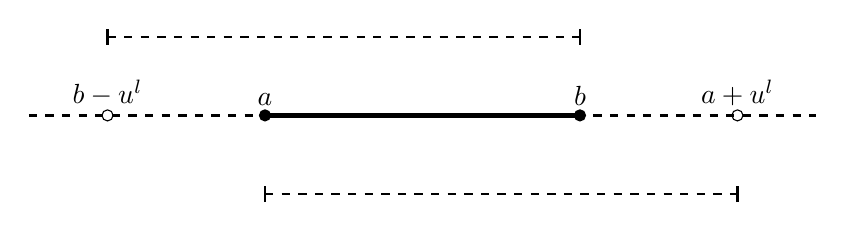
\begin{tikzpicture}
        \draw[dashed, black, thick] (-2,0) -- (4,0);
        \draw[black, thick] (-2,-0.1) -- (-2,0.1);
        \draw[black, thick] (4,-0.1) -- (4,0.1);
        
        \draw[dashed, black, thick] (-5,1) -- (5,1);
        \draw[black, ultra thick] (-2,1) -- (2,1);
 
        
        \draw[dashed, black, thick] (-4,2) -- (2,2);
        \draw[black, thick] (-4,1.9) -- (-4,2.1);
        \draw[black, thick] (2,1.9) -- (2,2.1);
        
        \draw [black] (-4,1) circle (2pt) node[anchor=south] {$b-u^l$};

        \filldraw [black] (-2,1) circle (2pt) node[anchor=south] {$a$};

        \filldraw [black] (2,1) circle (2pt) node[anchor=south] {$b$};

        \draw [black] (4,1) circle (2pt) node[anchor=south] {$a+u^l$};
    \end{tikzpicture}
    \caption{Illustration of generalisation to arbitrary intervals $[a,b]$ for range proofs}
    \label{fig:interval}
\end{figure}


\subsection{Bulletproofs}
The construction of bulletproofs presented in \cite{bulletProofs_theory} is presented. This construction is based on a inner-product argument. 
\subsubsection*{Notation}
The description and construction or bulletproofs requires some additional notation which will be presented here. First let lowercase bold font denote vectors, i.e $\mathbf{a}\in\mathds{F}$ is a vector with element $a_1,..,a_n \in \mathds{F}$, and uppercase bold font denote matrices, i.e $\mathbf{A}\in\mathds{F}^{n\times m}$ is a matrix and $a_{ij}$ the element of $\mathbf{A}$ at row $i$ and column $j$. Given this notation denote scalar multiplication with a vector as $\mathbf{b}=c\cdot \mathbf{a}\in\mathds{F}$, where $c\in\mathds{F}$ and $\mathbf{b}=(b_1,...,b_n)$ where $b_i=c\cdot a_i$. Denote the euclidean inner product of two vectors as $\langle \mathbf{a},\mathbf{b}\rangle$ and Hadamard product as $\mathbf{a}\circ \mathbf{b}$.

Further consider vector polynomials $p(X)$ of degree $d$ on the form $p(X)=\sum_{i=0}^d \mathbf{p_i}\cdot X^i\in\mathds{Z}_p^n[X]$, where the coefficients $\mathbf{p_i}\in\mathds{Z}_p^n$. The inner product of two vector polynomials, $l(X),r(X)$ is defined as, 
\begin{align*}
    \langle l(X),r(X)\rangle = \sum_{i=0}^d\sum_{j=0}^n \langle l_i,r_j\rangle \cdot X^{i+j}\in\mathds{Z}_p[X].
\end{align*}
The following is equivalent: evaluating two polynomials at $x$ then taking the inner product versus taking the inner product polynomial at $x$.

Let $\mathbf{a}||\mathbf{b}$ denote the concatenation of two vectors and for $0\leq l\geq n$ use python notation to denote sections of vectors such that $\mathbf{a}_{[:l]} = (a_1,...,a_l)$ and $\mathbf{a}_{[l:]} = (a_{l+1},...,a_n)$. 

For $k\in\mathds{Z}_p^*$ let $\mathbf{k}^n=(1,k,k^2,...,k^{n-1})$, i.e the vector containing the $n$ fist powers of $k$. 

Also let $\mathbf{g},\mathbf{h}\in\mathds{G}^n$ be two vectors. Given such a vector $\mathbf{g}$ and a vector $\mathbf{a}\in\mathds{Z}_p^n$ write $C= \mathbf{g}^\mathbf{a} = \prod_{i=1}^ng_i^{a_i}\in\mathds{G}$. $C$ can be interpreted as a commitment to the vector $\mathbf{a}$.

Remark that is this section $n$ denotes the dimension of the room not the number of clients, further remark that the dimension of the room is the length of the bit representation of the secret in the Pedersen vector commitment considered below. 

\subsubsection*{Inner product argument}
\label{sec:inner_prod}
The bulletproof construction is based on the inner product argument presented in this section. The inner product argument is a argument of knowledge of $\textbf{s},\mathbf{r}$ in a  Pedersen vector commitment $P_v=\mathbf{g}^\mathbf{s}\mathbf{h}^\mathbf{r}$ satisfying a given inner product. (To differ from the Pedersen vector commitment considered here and the Pedersen commitment in the range proofs the exponents in the commit are denoted $\mathbf{s},\mathbf{r}$ instead of $\sigma,R$, and the commitment by $P_v$) More formally the argument is a proof system of the statement,
\begin{align*}
    \{(\mathbf{g},\mathbf{h}\in\mathds{G}^n,P_v\in\mathds{G},c\in\mathds{Z}_p;\: \mathbf{s},\mathbf{r}\in\mathds{Z}_p^n) : \: P_v=\mathbf{g}^\mathbf{s}\mathbf{h}^\mathbf{r}\wedge\: c =\langle\mathbf{s},\mathbf{r}\rangle\}
\end{align*}
Which can be shown to be equivalent to a proof of the statement,
\begin{align*}
    \{(\mathbf{g},\mathbf{h}\in\mathds{G}^n,u,P_v\in\mathds{G};\: \mathbf{s},\mathbf{r}\in\mathds{Z}_p^n) : \: P_v=\mathbf{g}^\mathbf{s}\mathbf{h}^\mathbf{r}u^{\langle\mathbf{s},\mathbf{r}\rangle}\}.
\end{align*}

The construction to prove the inner product argument is presented in Construction \ref{alg:inner_product}. The construction presented is modified compared to the one presented in \cite{bulletProofs_theory} to be non-interactive using the Fiat-Shamir heuristic by \cite{ZKRP_Morais}.

\begin{algorithm}[H]
\caption{\textbf{: Inner-product argument}}
\textbf{Goal:} Given a Pedersen commitment $C=g^\sigma h^R$ and two parameters $u,l$, prove that the secret $\sigma=\sum_{j=0}^l \sigma_ju^j$ belongs to the interval $[0,u^l)$ without revealing anything else about $\sigma$.
\vspace{2pt}
\hline
\vspace{2pt}
\begin{itemize}
\item\text{\textbf{Prove} $(\mathbf{g},\mathbf{h},P_v=\mathbf{g}^s \mathbf{h}^r,c,\mathbf{r},\mathbf{s})\xrightarrow[]{}\textit{ proof}_{IP}=(\mathbf{g},\mathbf{h},P_v',u^x,\mathbf{s},\mathbf{r},\mathbf{l},\mathbf{r})$}\\
Let $x=\text{Hash}(\mathbf{g},\mathbf{h},P_v,c) \in\mathds{Z}_p^*$ and compute $P_v'= u^{x\cdot c}P$. Then define the two vectors $\mathbf{l},\mathbf{r}$.
\begin{itemize}
    \item If the dimension of the vectors $\mathbf{g},\mathbf{h},\mathbf{s},\mathbf{r}$ is one drop the bold font in the notation and publish the proof $\textit{ proof}_{IP}=(g,h,P_v',u^x,s,r,\mathbf{l},\mathbf{r})$.
    \item  Otherwise:  Let $n'=n/2$ and define  $c_L=\langle a_{[:,n']},b_{[n',:]} \rangle$ and $c_R=\langle a_{[n',:]},b_{[:,n']} \rangle$. Then use these variables to calculate $L=\mathbf{g}_{[n':]}^{\mathbf{a}_{[:n']}} \mathbf{h}_{[:n']}^{\mathbf{b}_{[n':]}} u^{c_L}$ and $R=\mathbf{g}_{[:n']}^{\mathbf{a}_{[n':]}} \mathbf{h}_{[n':]}^{\mathbf{b}_{[:n']}} u^{c_R}$. Further store the current values of $L,R\in\mathds{G}$, by appending them to the vectors $\mathbf{l}$ resp $\mathbf{r}$. Now update $x=\text{Hash}(L,R)$, and recalculate $\mathbf{g} = \mathbf{g}_{[:n']}^{x^{-1}}\mathbf{g}_{[n':]}^{x}$, $\mathbf{h} = \mathbf{h}_{[:n']}^{x}\mathbf{h}_{[n':]}^{x^{-1}}$ and the commitment $P'=L^{x^2}PR^{x^{-2}}$. Finally update the exponents $\mathbf{s},\mathbf{r}$ to $\mathbf{s} = \mathbf{s}_{[:n']}+\mathbf{s}_{[n':]}x^{-1}$ and $\mathbf{r} = \mathbf{r}_{[:n']}x^{-1}+\mathbf{r}_{[n':]}x$. Run the step \textbf{Prove}$(\mathbf{g},\mathbf{h},P_v',n',\mathbf{r},\mathbf{s})$ with the updated variables. Note that the vectors $\mathbf{g},\mathbf{h},\mathbf{s},\mathbf{r}$ now have the dimension $n'=n/2$, hence performing the recursion until one-dimensional vectors will require $log\:n$ iterations.
\end{itemize}
\item\text{\textbf{Verify} $(g,h,C,\textit{proof})\xrightarrow[]{}\{0,1\}$}\\
For $i\in\{0,log(n)\}$ put $n=n/2$ and $x=\text{Hash}(\bm{l}[i],\bm{r}[i])$, then update the vectors $\bm{g}$ and $\bm{h}$ as well as the  variable $P$ according to, $\bm{g}= \bm{g}_{[:,n]}^{x^{-1}}\bm{g}_{[n,:]}^{x}$, $\bm{h}= \bm{h}_l{[:,n]}^{x}\bm{h}_{[n,:]}^{x^{-1}}$ and $ P = L^{x^2}PR^{x^{-2}}  $. After iterating over all $i$ the dimension of the vectors $\bm{g},\bm{h}$ is one and we can drop the bold font. Accept if $c=\langle s,r\rangle$ and $P =g^sh^r$.

Accept if 
\end{itemize}
\label{alg:inner_product}
\end{algorithm}

%The setup phase of construction \ref{alg:inner_product} is intently left out since to avoid a trusted third party a \textit{Nothing up my sleeve} strategy will be used and is described separately in  section \ref{sec:NOMS}.
 


\subsubsection*{Inner product rang proof}
Based on the inner product argument  in this section the construction a range proof called  \textit{bulletproof}, will be described. This construction allows a prover, given a Pedersen commitment $C=g^\sigma h^R$ to convince a verifier that the secret $\sigma$ belongs to the interval $[0,2^n)$. To do this the prover needs to convince the verifier that:
\begin{itemize}
    \item $\bm{\sigma}\in\{0,1\}^n$ is the binary representation of $\sigma$, or equivalently that $\langle \bm{\sigma},\mathbf{2}^n\rangle = \sigma$.
    \item $\bm{\bar{\sigma}}$ is the component-wise complement of $\bm{\sigma}$. This is equivalent to show that $\bm{\bar{\sigma}}$ satisfies the two conditions: $\bm{\bar{\sigma}}\circ \bm{\sigma}=\bm{0}^n$ and $\bm{\bar{\sigma}} = \bm{\sigma} -\bm{1}^n \: \text{mod }2$.
\end{itemize}
These three equations can be rewritten and summarised in proving the following statement;
\begin{align}
    \big\langle \bm{\sigma} -z\cdot \bm{1}^n, \bm{y}^n\circ (\bm{\bar{\sigma}} + z \cdot\bm{1}^n) + z^2\cdot\bm{2}^n \big\rangle = z^2\cdot\sigma + \delta(y,z),
    \label{eq:range_non_zero}
\end{align}
where $\delta(y,z) = (z-z^2)\cdot\langle\bm{1}^n,\bm{y}^n\rangle-z^3\langle \bm{1}^n,\bm{2}^n\rangle\in\mathds{Z}_p.$.
The values $z$ and $y$ are either chosen at random from the set $\mathds{Z}_p$ by the verifier in an interactive construction or are the hash of other values in a non-interactive construction. Here a non-interactive construction will be considered, for further definition of the variables $z,y$ see Construction \ref{alg:bullet}.

If a inner product argument presented in Construction \ref{alg:inner_product} was used to prove the inner product defined in equation \eqref{eq:range_non_zero} it would leak information about $\sigma$, since information about the two vectors $\bm{\sigma},\bm{\bar{\sigma}}$ is revealed and they contain information about the binary representation of $\sigma$. Hence two new vectors $\bm{s}_1,\bm{s}_2$ are introduced and will serve as blinding vectors and help construct a zero-knowledge range proof even if the inner product argument is not a zero knowledge construction. Given this idea, the inner product in \eqref{eq:range_non_zero} is tweaked to include the two blinding vectors,
\begin{align}
     t(X) &= \langle  l(X),r(X)\rangle = t_0 + t_1\cdot X + t_2\cdot X^2\\
    l(X) &= \bm{\sigma} -z\cdot \bm{1}^n +\bm{s}_1\cdot X\\
    r(X) &= \bm{y}^n\circ (\bm{\bar{\sigma}} + z \cdot\bm{1}^n + \bm{s}_2\cdot X)+ z^2\cdot\bm{2}^n,\\
    \label{eq:range_zero}
\end{align}
Clearly $t_0 = z^2\cdot\sigma + \delta(y,z)$ which is equal to the right hand side of equation \eqref{eq:range_non_zero}. 